\chapter{FLC100 shield assembly}

\section{Introduction}
The FLC100 shield is an Arduino ``shield'' which operates at
\volt{3.3}. Do not attempt to use it with standard Arduino boards
which are operated at \volt{5}. The shield houses the XRF radio
module, the boost power supply (which creates the \volt{3.3} supply
for the microcontroller and radio) and the \volt{3.3} -- \volt{5} level
shifters.

There are both through-hole and surface mount versions of the boost
power supply. It is suspected that the through-hole version causes
\rfi\ since the radio module often fails to receive messages. This
problem was not apparent on the prototype board. The surface-mount
version has no such problems and is the option which should be
used. It is also cheaper and more efficient.

There is an option to fit a FLC100 sensor directly to the circuit
board. This option is not used because the FLC100 is slightly
temperature sensitive and better performance is obtained by
positioning the sensor below ground. Whilst the board provides an
option to fit an MCP3424 \adc\ and MAX619 charge-pump power supply they
are also fitted remotely, below ground, for reasons of temperature
stability.

\section{FLC100 shield version 1.0}

\begin{figure}
  \centering
  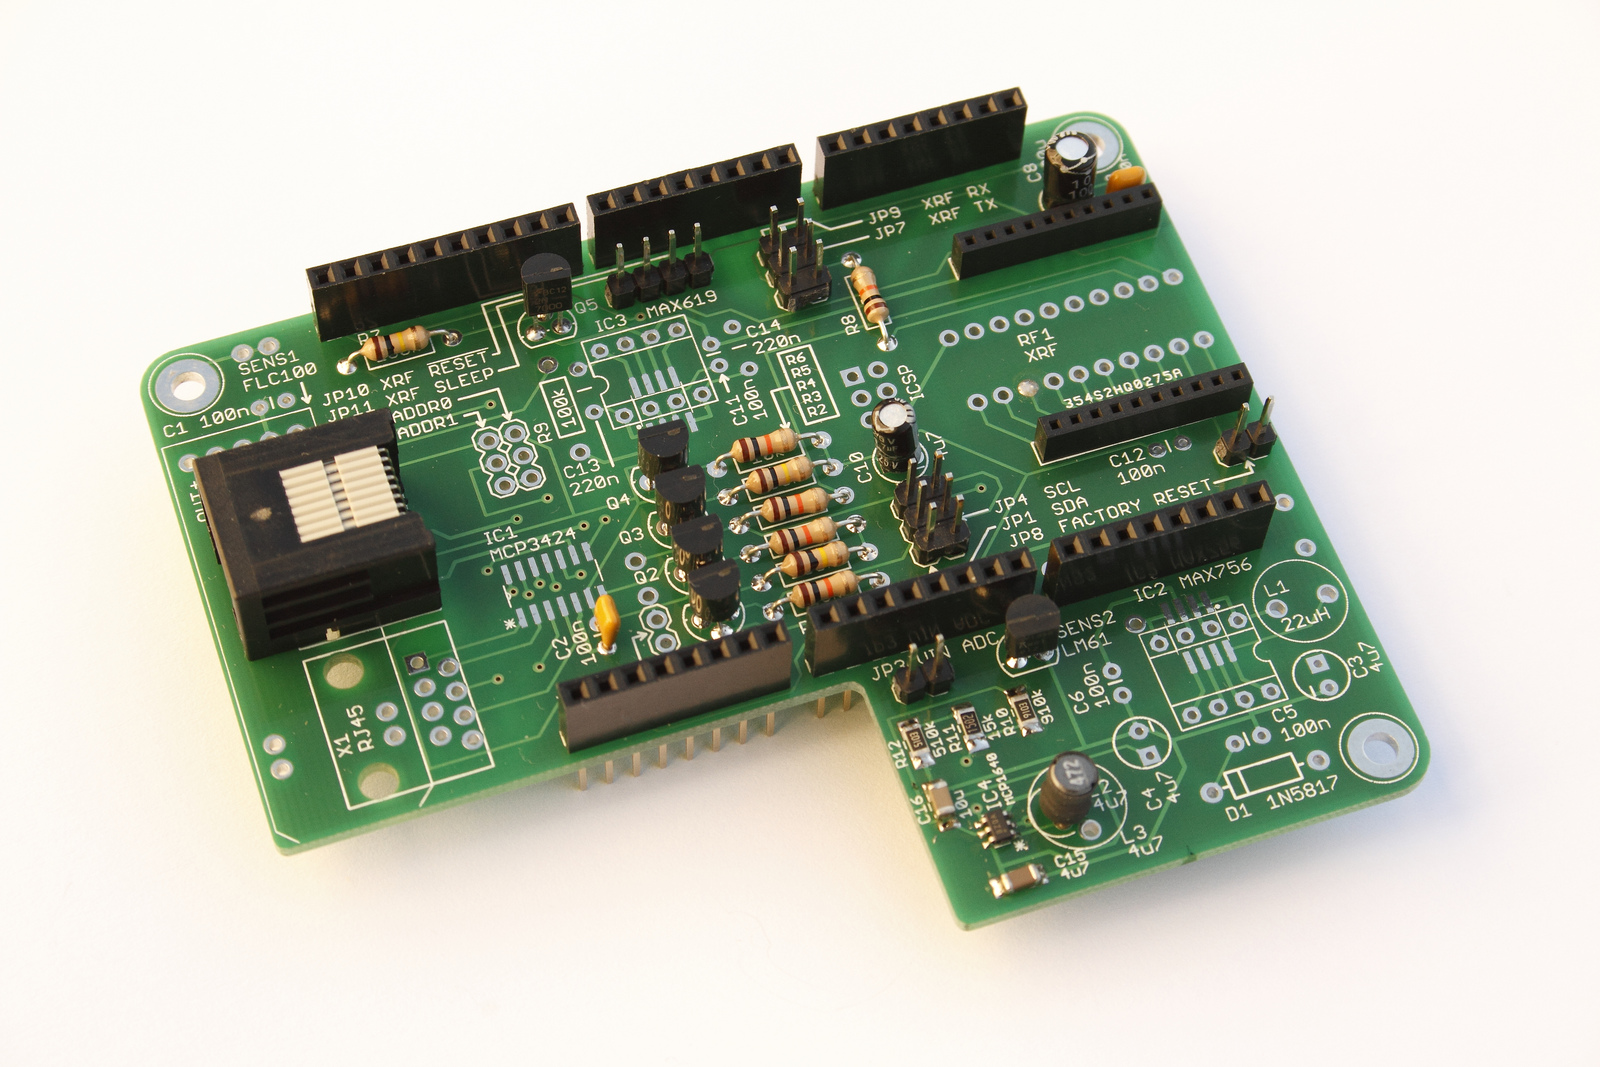
\includegraphics[keepaspectratio,width=\textwidth]{%
    images/flc100-shield}
  \caption[Completed FLC100 shield]{Completed FCL100 shield, except
    for fitting shunts onto the jumpers. %
    \photoCredit{Steve Marple}{\ccBySaTwo}{%
      http://www.flickr.com/photos/stevemarple/10787109594/}}
  \label{fig:flc100-v1.0}
\end{figure}

\subsection{Order of assembly}
\begin{buildorder}
\item IC4 (MCP1640).
\item R12 (\kohm{510}).
\item R11 (\kohm{15}).
\item R10 (\kohm{910}).
\item \SI{2}{\milli\metre} 10~way connectors for RF1. Ensure they are
  fitted flush to the \pcb.
\item C15 (\uF{4.7}).
\item C16 (\uF{10}).
\item R1, R3, R4, R6, R8 (\kohm{10}).
\item R2, R5, R7 (\kohm{100}).
\item C2, C7, C9 (\nF{100}).
\item C10 (\uF{4.7}).
\item C8 (\uF{100}).
\item L2 (\uH{4.7}). The shorter lead should be connected to pin~1,
  which is the hole nearest the edge of the \pcb. Although the
  orientation of inductors is normally ignored communication with the
  manufacturer revealed that the shorter lead indicates the start of
  the winding. This arrangement is preferred to help minimise \rfi.
\item Stacking connectors, five 8~way and one 10~way. Ensure they are
  fitted flush to the \pcb.
\item JP1, JP4 ($2 \times 3$ jumper).
\item JP7, JP9 ($2 \times 3$ jumper).
\item JP10, JP11 ($1 \times 4$ jumper).
\item JP3 ($1 \times 2$ jumper).
\item JP8 ($1 \times 2$ jumper).
\item X2, RJ45 connector.
\item Q1, Q2, Q3, Q4, Q5 (2N7000).
\end{buildorder}

Fit shunts to JP10, JP11, JP3. Fit shunts to JP7 and JP9, to the two
connectors furthest from the edge of the \pcb. \textbf{Do not fit the
  shunts so that they bridge between JP7 and JP9}.

If the microcontroller board has dedicated \itwoc\ connections (\eg
Calunium v2.0 or later), then no shunts should be fitted to JP1 and
JP4. If the microcontroller has \itwoc\ connections in the standard
Arduino Mega positions (\eg, Calunium v1.0, Arduino Mega, Arduino Mega
2560) then fit shunts to JP1 and JP4 to the two connectors closest to
C10, otherwise fit shunts to JP1 and JP4 to the two connectors closest
to the stacking connectors. \textbf{In no circumstances should the
  shunts bridge between JP1 and JP4}.

Leave JP8 open circuit. It is fitted only when the XRF1 radio module
must be forced to use the default factory configuration.

\begin{landscape}
  \begin{figure}[p]
    \centering
    \includegraphics[keepaspectratio,width=28cm,height=16cm]{%
      images/FLC100_shield_v1_0_sch}
    \caption{FLC100 shield v.~1.0 circuit diagram.}
    \label{fig:flc100-shield-v1.0-cct-diag}
  \end{figure}
\end{landscape}

